%!TEX root=../slr.tex
\section{Conduction}
\label{sec:conduction}
\subsection{The Search}
\label{sub:the_search}

SLR guideline literature \cite{Kitchenham2007,Tacconelli2010} recommend
that the first stage of any Systematic Literature Review be the search
for previous literature of this kind, since a recent systematic study
may render the execution of a new study disencourageable. In our case,
none of the several libraries used appeared to have any article of the
sort.

The search terms, derived in
Subsection~\ref{sub:research_questions_and_search_queries}, were run in
all libraries found in
Subsection~\ref{sub:library_selection_and_filter_definition}. The Google
Scholar search had the particularity of being run through a specialised
software called \textit{Publish or Perish}\cite{Harzing}, which allowed
the search results to be exported to a comma separated values file,
which made the process a lot easier, since it was then possible to work
the data directly in a spreadsheet program (Microsoft Excel, in this
particular case).

The conduction phase of our study followed the flowchart illustrated by
Figure~\ref{fig:flowchart}. Notice that Google Scholar is the first
library to be searched. This is motivated by the fact that the vast
majority of the articles were retrieved by Google's academic search
engine. In fact, GS-retrieved articles were so predominant that we had
to create a special EC, as described in
Subsection~\ref{sub:library_selection_and_filter_definition}.

\begin{figure}[htpb]
    \centering
    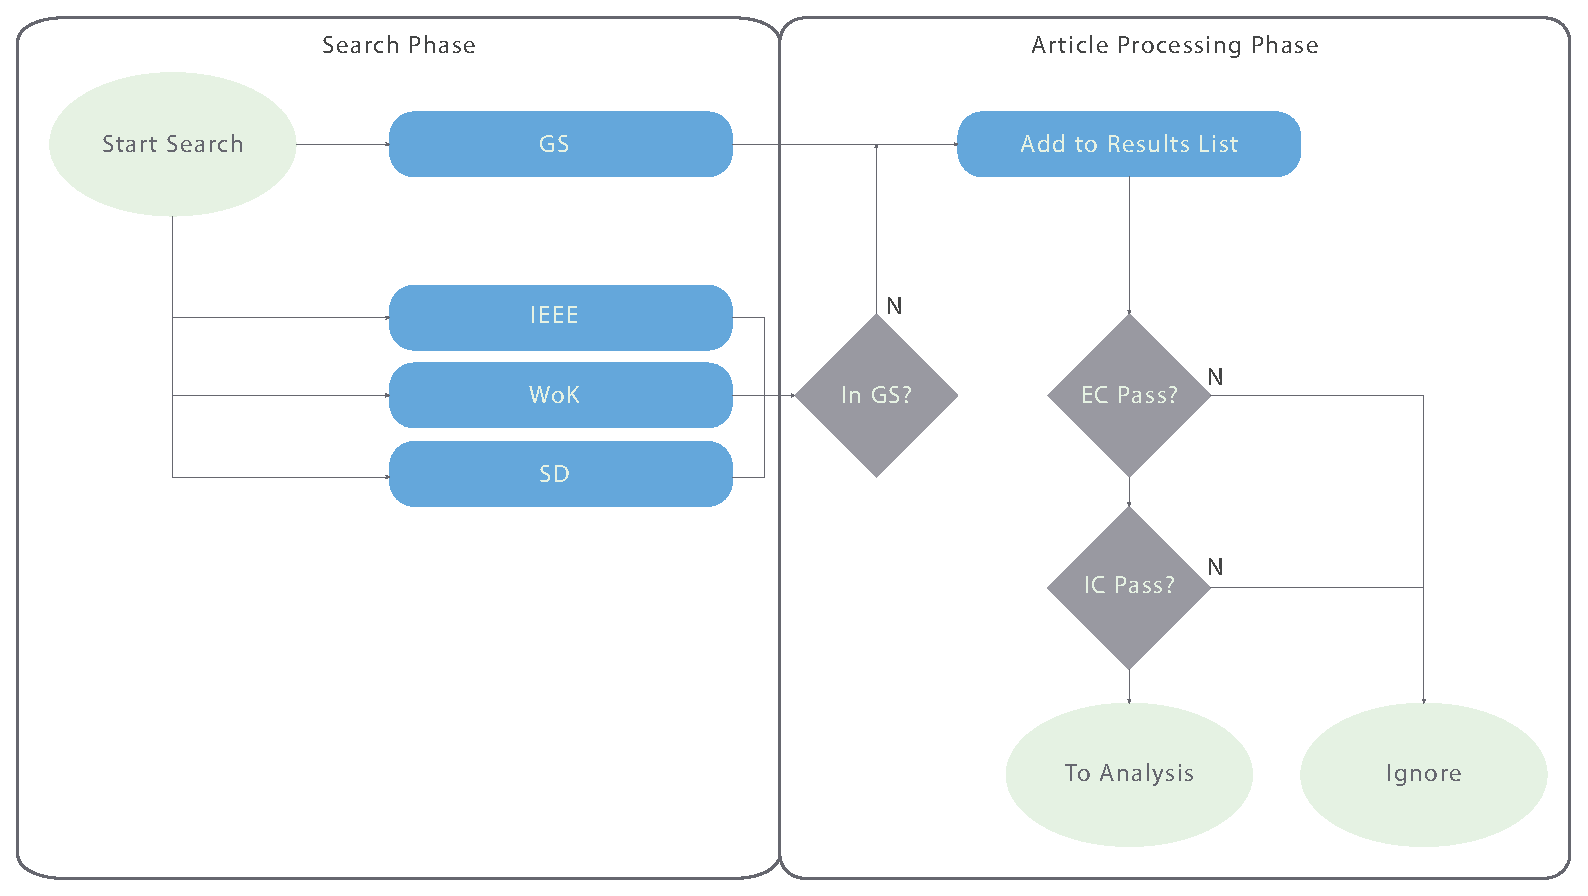
\includegraphics[width=\linewidth]{img/flowchart.eps}
    \caption{Conduction stage flowchart. Notice Google Scholar's
    prevalence.}
    \label{fig:flowchart}
\end{figure}

\subsection{Results and Discussion}
\label{sub:results_and_discussion}

\subsubsection{Presentation and analysis}
\label{ssub:result_presentation}

Our search returned 732 results, of which 709 were distinct
($\approx$97\%). Of these, 601 were journal articles ($\approx$82\%).
The vast majority of the results came from GS ($\approx$80\%, see
Figure~\ref{fig:results_distribution}).  Selection criteria (Inclusion
and Exclusion) application resulted in the exclusion of 701 results
($\approx$99\%), thus leaving 8 articles reaching the content analysis
stage (the attempt to answer the Research Question). A summary of these
findings can be seen in Table~\ref{tab:search_results}.

 \begin{table}[htb]
    \centering
    \caption{Search results. For a paper to reach the righmost column,
    which means it is selected, it must verify both IC1 and IC2 as well
    as none of the EC, ranging from EC1 to EC5.}
    \label{tab:search_results}
    \begin{small}
        \begin{tabularx}{\textwidth}{lcXXXXXXXr}%{@{}lllllllllr@{}}
            \toprule
             &  & \multicolumn{7}{c}{\textbf{Articles which trigger criteria}} &  \\ \midrule
            \textbf{Source} & \textbf{\# Articles} & \textbf{IC1} & \textbf{IC2} &
            \textbf{EC1} & \textbf{EC2} & \textbf{EC3} & \textbf{EC4} &
            \textbf{EC5} & \textbf{Rem. Articles} \\ \midrule
            GS & 576 & 455 & 142 & - & 25 & 82 & 53 & 18 & 8 \\
            IEEE & 116 & 116 & 1 & 0 & 0 & 1 & 1 & 0 & 0 \\
            WoK & 14 & 14 & 6 & 13 & 0 & 1 & 1 & 0 & 0 \\
            SD & 10 & 0 & 0 & 0 & 0 & 0 & 0 & 0 & 0 \\
            AGU & 16 & 1 & 1 & 1 & 1 & 1 & 1 & 0 & 1 \\ \midrule
                &  &  &  &  &  &  &  & \textbf{TOTAL} & 9 \\ \cmidrule(l){9-10}
        \end{tabularx}    
    \end{small}
\end{table}

\begin{figure}[htb]
    \centering
    \begin{tabular}[b]{lcr}
        \toprule
        \textbf{Library}&\textbf{\# Results}&\textbf{Percentage}\\
        \midrule
        \textbf{GS}&576&78.7\%\\
        \midrule
        \textbf{IEEE}&116&15.8\%\\
        \midrule
        \textbf{WoK}&14&1.9\%\\
        \midrule
        \textbf{SD}&10&1.4\%\\
        \midrule
        \textbf{AGU}&16&2.2\%\\
        \bottomrule
    \end{tabular}
    \qquad
    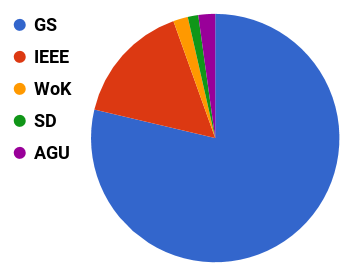
\includegraphics[width=0.4\textwidth]{img/new_results_distribution.png}
    \caption{Results distribution by
    library.}\label{fig:results_distribution}
\end{figure}

Table~\ref{tab:scores} presents the 8 selected articles. It categorises
them with respect to their covered topics and whether they are empirical
or theoretical in nature. The same table summarises article scores
according to the criteria defined in
Subsection~\ref{sub:quality_assessment}, and presents the the keys with
which we will refer to each article from this point forward.

The 8 papers averaged a score of 0,48 and a median score of 0,6. There
is a strong difference between the average and the median suggesting
that there are some outliers or some kind of clustering. Although this
is actually the case, it is statistically irrelevant, given the small
size of the sample.

\begin{table}[htb]
    \centering
    \caption{Scoring results for the selected articles. In the second
    column, a T means the article is theoretical and an E means the
    article is empirical.}
    \label{tab:scores}
    \begin{tabularx}{\textwidth}{lXXXXXr}
        \toprule
        \textbf{Key} & \textbf{Type} & \textbf{Alg.} & \textbf{Inst.} &
        \textbf{Soft.} & \textbf{Cit.} & \textbf{Score}\\
        \midrule
        Hartl2006~\cite{Hartl2006} & T & 1 & 0,4 & 0 & 0,5 & 0,73\\
        Laepple2004~\cite{Laepple2004} & T & 1 & 0 & 0 & 1 & 0,70\\
        Mettendorf2006~\cite{Mettendorf2006} & E & 0,4 & 1 & 1 & 0,25 & 0,57\\
        ODriscoll2003~\cite{ODriscoll2003} & T & 1 & 0 & 0 & 0,25 & 0,63\\
        Olaguer2017~\cite{Olaguer2017} & E & 0 & 0,2 & 0 & 0,25 & 0,07\\
        Poehler (unpub)~\cite{Poehler} & E & 0 & 0,4 & 0 & 0,25 & 0,11\\
        Pundt2005~\cite{Pundt2005} & E & 0,4 & 1 & 1 & 1 & 0,64\\
        Stutz2016~\cite{Stutz2016} & E & 0 & 1 & 1 & 0,25 & 0,33\\ 
        \bottomrule
    \end{tabularx}
\end{table}

% \begin{figure}[htb]
%     \centering
%     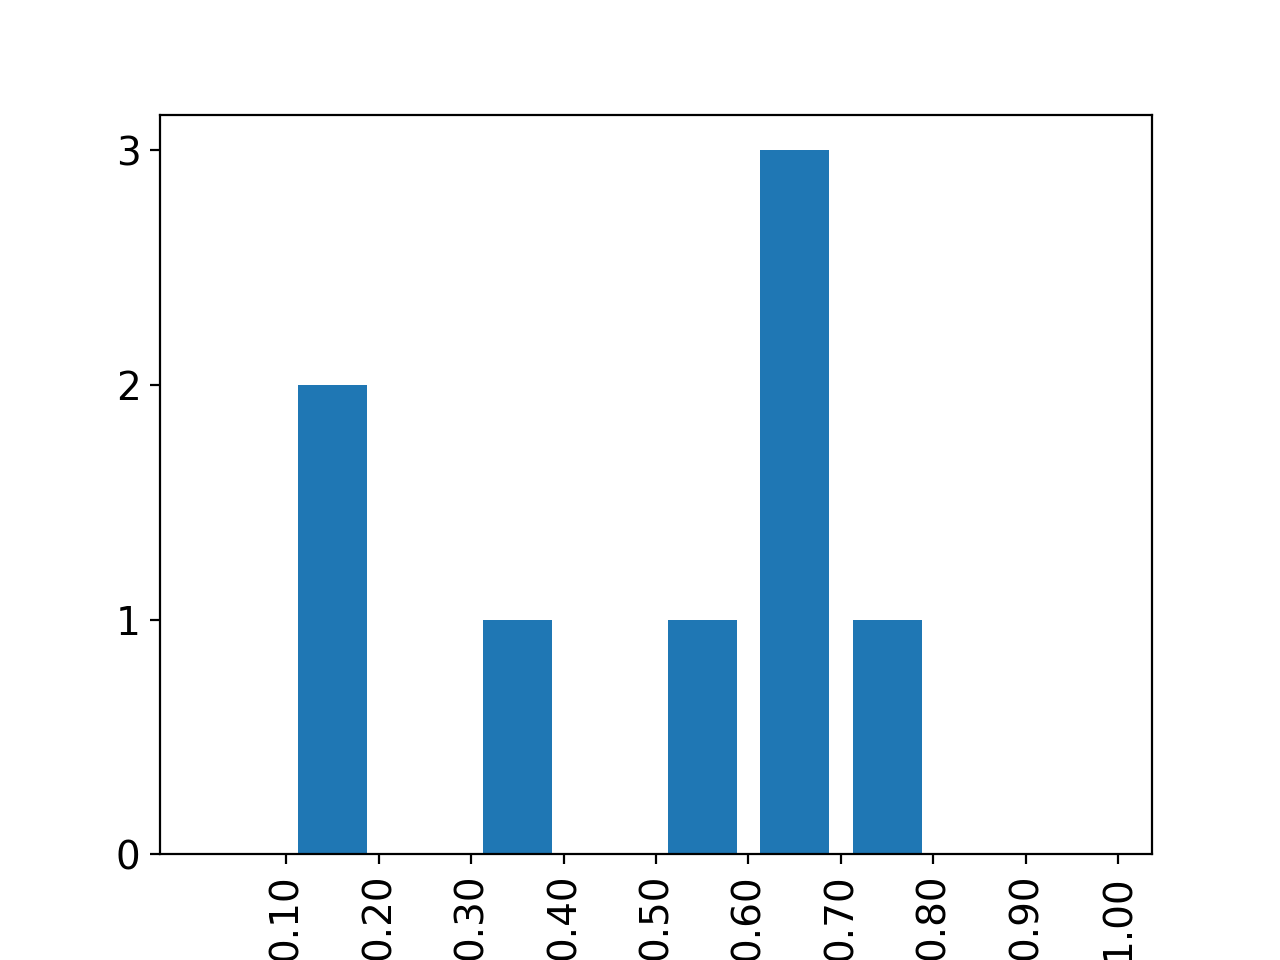
\includegraphics[width=\textwidth]{img/histogram.png}    
%     \caption{Score histogram for the articles in selection.}
%     \label{fig:score_histogram}
% \end{figure}

% \begin{table}[htb]
%     \centering
%     \caption{Article metrics: selection vs whole search.}
%     \label{tab:metrics}
%     \missingtable{Metrics table}
% \end{table}

\subsection{Discussion}
\label{sub:discussion}

In this subsection, we will use the 8 articles that were selected in
order to try and answer the Research Questions. For clarity, we will
approach with respect to the instrument, algorithm and software in a
separate manner.

Different articles present data in different ways, and with different
levels of detail. This has been taken into account in designing our
evaluation method, and it should also be observed when discussing
results. Therefore, our general approach in this subsection will be to
address the more detailed articles first and then complement that
information with what we can gather from the less detailed papers.

\subsubsection{Instrument}
\label{ssub:instrument}

Instrumentation description is present in 7 of the 8
(\cite{Hartl2006,Laepple2004,
Mettendorf2006,Olaguer2017,Poehler,Pundt2005, Stutz2016}) selected
articles. Stutz2016~\cite{Stutz2016}, Pundt2005~\cite{Pundt2005} and
Mettendorf2006~\cite{Mettendorf2006} present the highest level of
detail.

In Stutz2016~\cite{Stutz2016}, the authors used a newly developed Long
Path DOAS instrument for the study of atmospheric concentration of
Benzene, Toluenes and Xylenes. This instrument's main innovation is its
light source, which consists in a double LED (255nm and 265nm) assembly.
This system's telescope is a homebuilt telescope with a focal length of
120 cm and a 12 inch diameter aluminum coated main mirror, mounted on a
high accuracy motorised pan and tilt unit from Newark Systems. The
telescope is used both as emitter and receiver, therefore the system
needs a reflector. Stutz used a quartz corner cube reflector array,
with an individual reflector diameter of 57 mm and the number of
reflector ranging from 10 to 25 (depending on the path length). For
detection, the system relied on a UV-enhanced PIXIS 256 CCD detector
from Princeton Instruments on an Acton spectrometer with 300 grating and
$\approx$0,3 nm spectral resolution, which was stabilised to -35ºC.

Pundt2005~\cite{Pundt2005} was conducted during the BAB II motorway
campaign. The team was working with the goal of performing a tomographic
measurement of vehicle polution along a certain motorway between
Heidelberg and Mannheim. For that, they used an assembly of two
telescopes and eight reflectors, rendering a total of 16 light paths,
then used to perform a tomographic reconstruction of the trace gas
detection in that region. The telescopes used had a focal length of 150
and 80 cm, with respective diameters of 300 and 200 mm. Both assemblies
used Acton spectrometers. One used the Acton 500, with 0,5 nm spectral
resolution in the range between 295 and 375 nm; the other used an Acton
300, with 0,4 nm spectral resolution between 295 and 355 nm. In both
cases, the sensor used was a 1024 pixe Photo Diode Array (PDA),
thermally stabilised at -15ºC. The telescopes were pointed towards two
towers which beared the reflectors, set at heights of 10, 20, 30 and 40
m from the ground. The system's geometry and distances are shown in
Figure~\ref{fig:babii_geometry}.

\begin{figure}[htb]
    \centering
    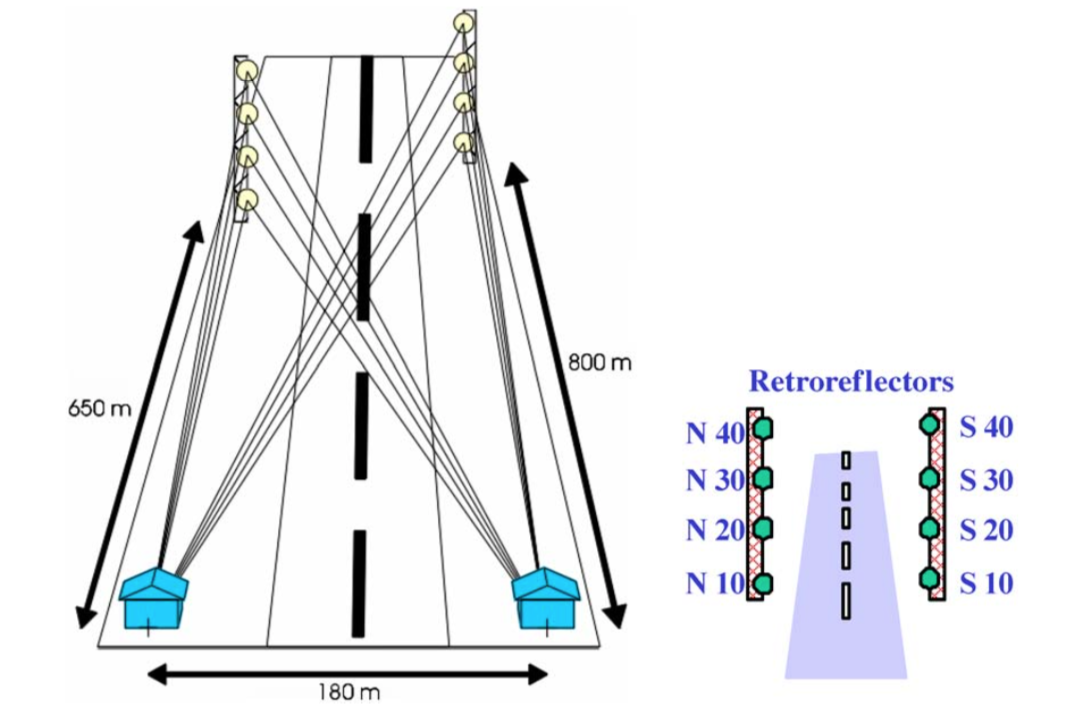
\includegraphics[width=0.8\linewidth]{img/babii_geometry.png}
    \caption{Schematic representation of the BABII campaign
    experiment~\cite{Pundt2005}.}\label{fig:babii_geometry}
\end{figure}

In Mettendorf2006~\cite{Mettendorf2006}, the authors validated
two-dimensional LP-DOAS tomography through an indoor experiment. To this
end, they have used three multibeam instruments, which consisted in a
telescope with a focal length of 1,5 m and 300 mm in diameter, which was
also used as emitter and receiver. The system used a broad spectrum
Xenon lamp as light source, though no details are given. The experiment
assembly included the careful positioning of plane mirrors and 6 cm
diameter corner cube reflectors, used to create a total of 39 light
paths (13 for each multibeam instrument). Telescope, mirror and
reflector positions are illustrated in Figure~\ref{fig:mettendorf_geom}.

\begin{figure}[htb]
    \centering
    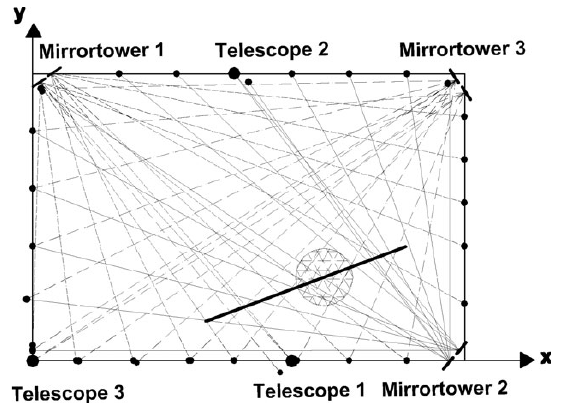
\includegraphics[width=0.8\linewidth]{img/mettendorf.png}
    \caption{Mettendorf2006~\cite{Mettendorf2006} experiment geometry,
    detailing position of telescopes (large filled dots), mirrors (small
lines in upper corners), reflectors (small dots along edges), test
samples (hatched circle), light paths (thin lines) and the movement path
for the sample (thick diagonal line).}\label{fig:mettendorf_geom}
\end{figure}

As for the other 4 less detailed instrument description, three
(Hartl2006~\cite{Hartl2006}, Poehler~\cite{Poehler} and
Laepple2004~\cite{Laepple2004}) are from the same group as
Pundt2005~\cite{Pundt2005} and Mettendorf2006~\cite{Mettendorf2006}, and
therefore use the same or similar hardware.
Olaguer2017~\cite{Olaguer2017}, on the other hand, is the companion
paper of Stutz2016~\cite{Stutz2016}, and therefore gives a description
of the same instrumentation, though in a less detailed manner.

\subsubsection{Algorithm}
\label{ssub:algorithm}

The reconstruction algorithm is the most important part of our study, as
we already demonstrated by the weight it is given in our quality
evaluation model (see Subsection~\ref{sub:quality_assessment}).
Algorithm descriptions are present in 6 of the 8 selected
articles:~\cite{Hartl2006, Laepple2004, Mettendorf2006, ODriscoll2003,
Olaguer2017, Pundt2005}. The most complete descriptions are featured in
Hartl2006~\cite{Hartl2006}, Laepple2004~\cite{Laepple2004} and
ODriscoll2003~\cite{ODriscoll2003}.
Mettendorf2006~\cite{Mettendorf2006}, Olaguer2017~\cite{Olaguer2017} and
Pundt2005~\cite{Pundt2005} approach the reconstruction algorithms with
less emphasis or in a less detailed way.

In Hartl2006~\cite{Hartl2006}, the research team describe their
discretisation process, reconstruction methods, grid translation methods
and error estimation and quality assessment, with the greatest level of
detail being given to the latter.

The paper also focuses in the comparison SIRT and ART results for the
test samples, which consisted in up to four Gaussian concentration
profiles, which were randomly arranged in a 100x100 (a.u.) test field,
in six different geometries and  with up to 36 known light paths.

Furthermore, Hartl2006~\cite{Hartl2006} discusses how the choice of the
reconstruction grid affects both the reconstruction error and
reconstruction area integrals, the possibility of the existence of
background concentration influencing equation constraints and
reconstruction results, and how the whole system would behave were its
geometry any different, namely regarding light paths and number of
telescopes. 

The next algorithm-oriented paper is Laepple2004~\cite{Laepple2004}. In
this article, the group discussed several discretisation approaches,
their drawbacks and advantages. Still on discretisation, they approach
the problem of resolution, and the necessary balance between physical
accuracy and the need for \emph{a priori} information which arises from
increasing it. Afterwards, the group presents some strategies for
solving the linear system that results from discretising the
concentration field and how to take error into account.

For their reconstructions, the group chose to adapt ART, SIRT, and SART
. These adaptations were described and detailed in the article's third
section, before the error estimation procedures adopted in their case.
Finally, the team presents how they chose to optimise reconstruction in
several aspects, including the generation of test plumes and
optimisation for the BABII campaign, which was the parent project of
this article. 

ODriscoll2003~\cite{ODriscoll2003} also covers the algorithm
extensively. While this paper is considerably shorter that the previous
two, it provides a detailed (on an iteration basis) description for ART
and SIRT. In addition, and perhaps of greater interest, the paper's
authors suggest a different approach to solving the reconstruction
matrix, different from the algebric methods already presented: an
evolutionary algorithm.

An evolutionary algorithm is a mathematical method of solving complex
problems, which mimics or is in any form based on the process of natural
selection. These algorithms have, according to the paper's authors and
their references, been shown to be extraordinarily powerful.

The research team have applied a Differential Evolution algorithm to the
reconstruction process and provide a detailed description of how they
have done this.

The other two articles which mention the algorithm are
Mettendorf2006~\cite{Mettendorf2006} and Pundt2005~\cite{Pundt2005}.
Both these studies were conducted under the same project as
Laepple2004~\cite{Laepple2004} and Hartl2006~\cite{Hartl2006} and
therefore their algorithm descriptions and methods draw heavily on
these two studies.


\subsubsection{Software}
\label{ssub:software}

Of the 8 selected articles, only 3 mention the software used. Even these,
do not go into any detail of the reasons that led to that specific
usage. 

In Mettendorf2006~\cite{Mettendorf2006}, the team used TOMOLAB
for the calculation of the modelled column densities of their
experiment. In Pundt2005~\cite{Pundt2005}, spectral analysis was
performed using the \emph{MFC Software}. Finally,
Stutz2016~\cite{Stutz2016} used the DOASIS software for control and
automation purposes, and does not explicitly mention its use for
spectral analysis purposes, although this is likely.

\subsubsection{General Observations}
\label{ssub:general_observations}

While this is not a part of the discussion \emph{per se}, we believe it
makes sense to make some general observations about the data which wwe
had to analyse.

The first important mention is the BABII campaign. This study, which ran
in 2001 and aimed to quantify polution from the A656 motorway between
Heidelberg and Mannheim produced a significant part of the literature
which we analysed.

Another point which should be addressed is that all DOAS tomography
efforts detected in this search were based on active DOAS technology.
This only means that the DOAS systems all employed an artificial light
as a light source.

A final remark is due to the prevalence of algebric methods for
solving the discretisation and reconstruction problem, namely ART, SART
and SIRT. 

\subsection{Validity Threats}
\label{sub:validity_threats}

When writing an MS or an SLR, authors always have to analyse their
findings and methods in order to mitigate potential sources of error or
lack of validity. This is called a validity threat analysis.

There are two main families of validity threats. They can be internal,
i.e., they come from the methods employed used in conducting the study;
or external, which means that the threat comes from the applicability
(or lack thereof) of the effects observed in the study, outside of its
scope.

On the level of internal validity of our study, two main observations
come to mind:
\begin{description}
    
    \item[Relevant papers left out] The very low number of found studies
        could be an indication that our inclusion and exclusion filters
        were set in a too restrictive manner. 
        
        It could also happen that some relevant papers were not found
        due to being written in such a way that the libraries' search
        engines did not find them with our search phrase. This same
        problem would also occur if for some reason, an important
        library was left out of the study, and therefore not searched.

        We mitigate all these risks by selecting a purposefuly broad
        search phrase, by using powerful general search engines (eg.
        Google Scholar) and by running several undocumented test-runs
        with other search phrases.

        A common strategy used for tackling this kind of threat is to
        extend the study through snowballing. In our case, we have opted
        to not perform this operation because of the very high
        cross-reference pattern between studies which we have found.
    
    \item[Quality of selected papers] While it is true that we do not
        have any control over the quality of the articles rendered by
        the search engines, and there is no standard regarding it, we
        must address the issue that it entails. We have tried to
        mitigate this risk, as far as we can, by using strict and strong
        selection criteria in systematic fashion (see
        Section~\ref{sec:methods}).

\end{description}

On the external threat plane, we contend with the applicability of our
findings outside our study. We have tackled this issue by trying to
remaining focused only to the techonologic aspect of the Tomographic
DOAS technique, both in respect to its instrumentation and to the
mathematical methods involved.

With this in mind, and even if the internal validity threats were all
verifiably concerning, this study's finding are of great use to anyone
wanting to understand how the field is working or wishing to design and
build an analysis system.
